\documentclass[conference, a4paper]{IEEEtran}
\IEEEoverridecommandlockouts
% The preceeding line is only needed to identify funding in the first footnote. If that is unneeded, please comment it out.
\usepackage{cite}
\usepackage{amsmath,amssymb,amsfonts}
\usepackage{algorithmic}
\usepackage{algorithm}
\usepackage{graphicx}
\usepackage[font=footnotesize]{caption}
\usepackage{textcomp}
\usepackage{xcolor}
\usepackage{url}
\usepackage{booktabs}
\usepackage{balance}
\usepackage{tikz}
\graphicspath{{images/}}
\setlength{\parskip}{6pt}
\setlength{\floatsep}{0pt}
\setlength{\textfloatsep}{6pt}
\setlength{\intextsep}{6pt}
\usepackage{titlesec}
\titlespacing*{\section}{0pt}{8pt}{4pt}
\titlespacing*{\subsection}{0pt}{6pt}{3pt}
\titlespacing*{\subsubsection}{0pt}{4pt}{2pt}
\usetikzlibrary{arrows.meta, shapes, positioning}
\usepackage{geometry}
\geometry{
  a4paper,
  top=2cm,
  bottom=2.5cm,
  left=1.6cm,
  right=1.6cm,
}

\def\BibTeX{{\rm B\kern-.05em{\sc i\kern-.025em b}\kern-.08em
    T\kern-.1667em\lower.7ex\hbox{E}\kern-.125emX}}
\begin{document}

\title{EcoHaul: A Smart Waste Management System Using a Dynamic Priority and Efficient Truck Dispatch Algorithm}

\makeatletter
\def\@IEEEauthorblockNfont{\fontsize{11pt}{13pt}\selectfont}
\def\@IEEEauthorblockAfont{\fontsize{10pt}{12pt}\selectfont}
\makeatother

\author{\IEEEauthorblockN{Atahan Düryaz}
\IEEEauthorblockA{\textit{Dept. of Computer Engineering} \\
\textit{Yeditepe University, Istanbul, Türkiye }\\
atahan.duryaz@std.yeditepe.edu.tr}
\and
\IEEEauthorblockN{Sebnem Baydere}
\IEEEauthorblockA{\textit{Dept. of Computer Engineering} \\
\textit{Yeditepe University, Istanbul, Türkiye }\\
sbaydere@yeditepe.edu.tr}
}

\maketitle

\begin{abstract}
Urban waste collection at city scale suffers from two structural problems: overflow risk in high-traffic areas that creates public-health hazards, and the chronic inefficiency of fixed-route collection that dispatches trucks to partially filled bins, wasting fuel and generating avoidable emissions. This paper presents EcoHaul, an AI-driven smart waste management system that addresses both problems through a Dynamic Priority and Efficient Truck dispatch (DPET) algorithm. EcoHaul couples a six-layer DPET pipeline---traffic modelling, predictive bin scoring, bin selection, mass-aware route optimization, route-efficiency validation, and dispatching---with a K-means/ETF fill predictor and a parallel dual-world simulation that runs DPET and a fixed-route baseline under identical conditions over 3{,}424 real bin locations from the Dublin City Council open dataset. A unified REST API lets physical ESP32 and ultrasonic sensors share the same endpoints as the simulation. Across one-year simulations, DPET improves system efficiency by about 30 percent, reduces fuel and carbon dioxide emissions by about 28 to 29 percent and operational cost by about 39 percent, while using 40 percent fewer trucks and 42 percent fewer trips than greedy and 2-opt baselines. A rule-based anomaly detector reaches an overall accuracy of 97.6 percent across six categories.
\end{abstract}

\renewcommand{\IEEEkeywordsname}{Keywords}
\begin{IEEEkeywords}
\itshape smart waste management, IoT, vehicle routing, dispatch optimization, fill prediction, digital twin
\end{IEEEkeywords}

\section{Introduction}
Waste management is among the most expensive recurring public services for large cities. Over the last three decades, urban population growth and rising per-capita waste have placed mounting pressure on collection systems that were designed for static demand. This pressure is not only logistic: it spans public health, environmental pollution, traffic, carbon emissions, and the annual fuel and operational budget.

Traditional collection follows predetermined fixed routes on a fixed timetable. Because routes are not driven by the actual fill level of the bins, trucks visit the same stops every day regardless of demand. Yet real fill levels are highly non-uniform: a bin next to a shopping centre may reach a critical level within hours, while a peripheral bin may take days. Fixed routes cannot adapt to this variability, which produces a dual inefficiency. First, \textit{overflow}: bins in high-traffic zones overflow before the scheduled truck arrives, causing pollution and health hazards. Second, \textit{under-utilization}: trucks are dispatched to half-empty bins, burning fuel and emitting CO\textsubscript{2} that could be avoided.

Formally, the problem is a dynamic, time-windowed variant of the Capacitated Vehicle Routing Problem (CVRP), in which one must service $N$ containers while minimising total cost (distance, fuel, emissions) without allowing additional overflow. EcoHaul attacks this problem with real sensor data, a dispatch algorithm, and a fill-prediction module integrated into a single dashboard. The system is grounded on a public dataset of 3{,}424 real bin locations in Dublin, Ireland. Its most distinctive feature is a \textit{parallel dual-world simulation} that runs two strategies---the proposed DPET algorithm and a conventional daily fixed route---on the same events and environment, providing a fair A/B comparison. The main contributions of this work are fourfold: (1) DPET, a six-layer dynamic dispatch algorithm that fuses predictive bin scoring with a mass-aware, physics-grounded routing cost; (2) a parallel dual-world simulation framework that benchmarks any dispatch policy against a baseline under identical stochastic conditions; (3) a lightweight K-means/ETF fill predictor that enables proactive dispatch without offline training; and (4) a unified REST interface that lets the same backend drive both the simulation and physical ESP32 sensors. The remainder of this paper reviews related work (Section~II), describes the system architecture (Section~III) and the DPET algorithm (Section~IV), summarises the implementation (Section~V), reports the experimental evaluation (Section~VI), and concludes (Section~VII).

\section{Related Work}
Four areas of prior work shaped EcoHaul's design: IoT-driven waste sensing, vehicle routing for collection, fill prediction, and smart-city simulation.

IoT-based bin monitoring has been an active field since the early 2010s, the core idea being to transmit fill state over a wireless link to a control centre. Gutierrez et al.~\cite{gutierrez2015} built an early ultrasonic, web-based system and showed that routing trucks only to bins above a fill threshold can cut cost by up to 40\%; their simple HTTP-based telemetry inspired EcoHaul's REST design. Arebey et al.~\cite{arebey2012} used camera images and Gray-Level Co-occurrence Matrix features for contactless level detection; EcoHaul targets the same contactless goal more cheaply with ultrasonic sensing. Pardini et al.~\cite{pardini2018} surveyed IoT waste solutions and stressed that low power and durability are decisive for outdoor ESP32-class hardware---requirements EcoHaul's firmware addresses with deep-sleep and RTC-memory persistence. Commercial Bigbelly solar bins, which already report fill levels in real time and appear in the Dublin dataset, confirm that the modelled scenario is realistic.

For routing, waste collection is a variant of the CVRP, a known NP-hard problem first formalised by Dantzig and Ramser~\cite{dantzig1959}; its intractability motivates heuristic and metaheuristic solutions. Christofides' heuristic~\cite{christofides1976} provides a $3/2$ worst-case guarantee for the TSP and underpins EcoHaul's use of 2-opt: EcoHaul builds an initial tour with the nearest-neighbor heuristic and refines it with 2-opt. Crucially, Akhtar et al.~\cite{akhtar2017} proposed a \textit{mass-dependent} fuel-consumption model for CVRP, showing that accounting for load when computing cost is essential. This motivates EcoHaul's mass-aware routing, in which the per-segment cost is

\begin{equation}
  C_{ij} = \bigl(m_{\text{base}} + m_{\text{current}}\bigr)\, d_{ij} + P_{\text{stop}},
  \label{eq:mass_aware}
\end{equation}

where $m_{\text{base}}=12{,}000$~kg is the empty truck mass, $m_{\text{current}}$ is the accumulated load, $d_{ij}$ is the inter-stop distance, and $P_{\text{stop}}$ is a service penalty. Rooted in $F=m\cdot a$, a heavier vehicle needs more force to accelerate; unlike distance-only heuristics, this yields a cost model closer to real fuel use.

For prediction, reactive systems act only after a bin is critically full, whereas proactive systems predict fill rate to prevent overflow. Anagnostopoulos et al.~\cite{anagnostopoulos2015} proposed a queue-based dynamic allocation framework and observed that bins in the same geographic cluster share filling characteristics; this directly motivates EcoHaul's K-means assignment of 3{,}424 bins into 12 regions for reliable regional prediction. Malapur and Pattanshetti~\cite{malapur2017} used gradient-boosted trees trained on fill data, outperforming threshold methods but requiring periodic retraining. For a continuously running simulation, EcoHaul instead uses a lightweight sliding-window estimate over recent fill cycles that needs no offline training.

Finally, EcoHaul's parallel-world simulation is a digital-twin approach: a digital replica of a physical system used to run what-if scenarios. Grieves and Vickers~\cite{grieves2017} introduced the digital-twin concept that pairs a physical and a digital entity with data flowing between them. EcoHaul is effectively a digital twin of the Dublin collection network and provides a controlled environment for a rigorous fixed-route-versus-DPET comparison that would be impossible in the field. Zanella et al.~\cite{zanella2014} defined a foundational IoT architecture for smart cities; following their interoperability principles, EcoHaul exposes both physical ESP32 sensors and the simulation through a single REST interface, enabling gradual hardware roll-out.

\section{System Architecture}
EcoHaul is a full-stack application built on a strictly layered, modular architecture (Fig.~\ref{fig:layers}). From bottom to top the five layers are a PostgreSQL/PostGIS database, an algorithm layer (DPET, fill predictor, anomaly detection), a dual-world simulation engine, a REST API, and a visualization dashboard. Each layer communicates only with its immediate neighbours through well-defined interfaces, so a layer can be developed, tested, and replaced in isolation without affecting the rest of the system; for instance, the pure algorithmic logic in Layer~2 is unit-tested independently of the asynchronous simulation loop in Layer~3, and the same REST contract in Layer~4 serves both the simulation and the physical IoT devices. This separation of concerns is what allows new dispatch policies or anomaly rules to be added without touching the data or presentation layers. The runtime data flow between the main components during a single dispatch cycle is shown in Fig.~\ref{fig:arch}.

\begin{figure}[t]
\centering
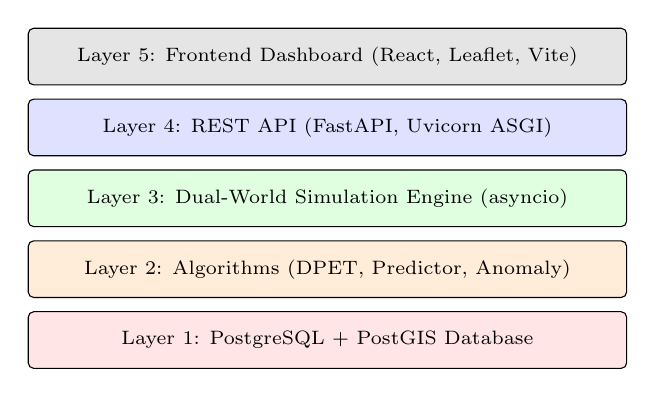
\begin{tikzpicture}[
  layer/.style={rectangle, draw, rounded corners=2pt, minimum width=7.6cm,
                minimum height=0.72cm, text centered, font=\scriptsize}
]
\node[layer, fill=gray!20]   at (0,3.6) {Layer 5: Frontend Dashboard (React, Leaflet, Vite)};
\node[layer, fill=blue!12]   at (0,2.7) {Layer 4: REST API (FastAPI, Uvicorn ASGI)};
\node[layer, fill=green!12]  at (0,1.8) {Layer 3: Dual-World Simulation Engine (asyncio)};
\node[layer, fill=orange!15] at (0,0.9) {Layer 2: Algorithms (DPET, Predictor, Anomaly)};
\node[layer, fill=red!10]    at (0,0.0) {Layer 1: PostgreSQL + PostGIS Database};
\end{tikzpicture}
\caption{EcoHaul five-layer system architecture; each layer interacts only with its immediate neighbours.}
\label{fig:layers}
\end{figure}

\begin{figure}[t]
\centering
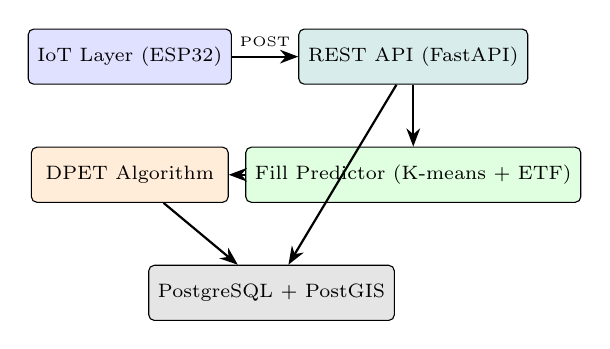
\begin{tikzpicture}[
  box/.style={rectangle, draw, rounded corners=2pt, minimum width=2.5cm,
              minimum height=0.7cm, text centered, font=\scriptsize},
  arrow/.style={-{Stealth}, thick}
]
\node[box, fill=blue!12]   (iot)  at (0,0)      {IoT Layer (ESP32)};
\node[box, fill=teal!15]   (api)  at (3.6,0)    {REST API (FastAPI)};
\node[box, fill=green!12]  (ml)   at (3.6,-1.5) {Fill Predictor (K-means + ETF)};
\node[box, fill=orange!15] (dpet) at (0,-1.5)   {DPET Algorithm};
\node[box, fill=gray!20]   (db)   at (1.8,-3.0) {PostgreSQL + PostGIS};
\draw[arrow] (iot)  -- node[above,font=\tiny]{POST} (api);
\draw[arrow] (api)  -- (ml);
\draw[arrow] (ml)   -- (dpet);
\draw[arrow] (dpet) -- (db);
\draw[arrow] (api)  -- (db);
\end{tikzpicture}
\caption{EcoHaul component interaction: telemetry from the IoT layer reaches the REST API, triggers the predictor and DPET, and is persisted in PostgreSQL/PostGIS.}
\label{fig:arch}
\end{figure}

\subsection{Dataset}
The primary dataset is the Dublin City Council public bin-location dataset~\cite{dcc2023}, summarised in Table~\ref{tab:dataset}. It provides 3{,}424 georeferenced bins with type and zone metadata. Coordinates are converted from Irish Transverse Mercator (EPSG:2157) to WGS84 (EPSG:4326) for web mapping and stored as PostGIS \texttt{POINT} geometry, enabling efficient spatial queries such as ``bins within 100\,m of a truck.'' Because the raw data contains only coordinates, the simulation engine synthesises realistic fill behaviour using zone type and statistically weighted distributions: fast (Label~A, 12--16\%/h), medium (Label~B, 4--8\%/h), and slow (Label~C, 0.5--1.5\%/h) bins, combined with five district archetypes.

\begin{table}[t]
\centering
\caption{Dublin City Council public bin dataset.}
\label{tab:dataset}
\footnotesize
\begin{tabular}{ll}
\toprule
\textbf{Feature} & \textbf{Value} \\
\midrule
Total records   & 3{,}424 waste containers \\
Original CRS    & Irish Transverse Mercator (EPSG:2157) \\
Web CRS         & WGS84 (EPSG:4326) \\
Coverage        & Dublin city centre and surroundings \\
Centre          & 53.34$^\circ$N, 6.27$^\circ$W \\
Container types & Cast Iron, Bigbelly Solar, Class A/B, Dog Waste \\
\bottomrule
\end{tabular}
\end{table}

\subsection{Layered Components}
\textbf{Layer~1 (Database)} stores the full system state in PostgreSQL with PostGIS. \textbf{Layer~2 (Algorithms)} holds the pure logic---DPET, median filtering, ETF prediction, anomaly detection---testable in isolation. \textbf{Layer~3 (Simulation Engine)} runs an \texttt{asyncio} event loop with two \texttt{WorldState} objects: a DPET world and a fixed-route world that runs a precomputed 2-opt tour at 06:00 daily. Both worlds share identical bin data and fill rates, so the only difference is the dispatch strategy. \textbf{Layer~4 (REST API)} is a FastAPI/Uvicorn server through which the frontend, the simulation, and physical ESP32 devices communicate. \textbf{Layer~5 (Frontend)} is a React/Leaflet dashboard that visualises bins, trucks, KPIs, anomalies, and simulation controls in real time.

\section{The DPET Algorithm}
DPET (\texttt{dpet.py}) converts the current bin states into an optimized dispatch plan through a six-layer pipeline, summarised in Algorithm~\ref{alg:dpet}. Each invocation scores every active bin, selects the most urgent candidates, packs them into capacity-bounded routes, optimizes those routes for fuel, rejects the inefficient ones, and finally hands the survivors to the fleet. The six layers are detailed below.

\begin{algorithm}[t]
\caption{DPET dispatch cycle (executed every simulation hour)}
\label{alg:dpet}
\begin{algorithmic}[1]
\REQUIRE bin states $B$, active fleet count, hour $h$, depot location
\ENSURE set of approved dispatch routes $R$
\STATE $T \gets$ \textsc{TrafficScore}($h$) \COMMENT{Layer 1}
\FORALL{bin $b \in B$}
  \STATE $s_b \gets 0.40\,s_{\text{fill}} + 0.35\,s_{\text{ETF}} + 0.12\,s_{\text{traffic}} + 0.08\,s_{\text{density}} + 0.05\,s_{\text{prox}}$ \COMMENT{Layer 2}
\ENDFOR
\STATE $C \gets$ bins of $B$ passing the fill/ETF thresholds \COMMENT{Layer 3}
\STATE sort $C$ by score $s_b$ in descending order
\IF{$|C| <$ \textsc{MinDispatch} \textbf{and} $C$ has no urgent bin}
  \RETURN $\emptyset$
\ENDIF
\STATE $R \gets \emptyset$
\FORALL{chunk of at most \textsc{MaxStops} bins taken from $C$}
  \STATE $route \gets$ \textsc{NearestNeighbor}($chunk$, $depot$) \COMMENT{Layer 4}
  \STATE \textsc{TwoOptMassAware}($route$) \COMMENT{minimise Eq.~\eqref{eq:mass_aware}}
  \STATE $\eta \gets |route| / \mathrm{dist}(route)$ \COMMENT{Layer 5}
  \IF{$\eta \geq 0.20$ \textbf{or} \textsc{IsUrgent}($chunk$)}
    \STATE $R \gets R \cup \{route\}$
  \ENDIF
  \IF{$|R| \geq$ available trucks}
    \STATE \textbf{break}
  \ENDIF
\ENDFOR
\RETURN $R$ \COMMENT{Layer 6: dispatch}
\end{algorithmic}
\end{algorithm}

\subsection{Layer 1: Traffic Model}
Each simulation hour receives a traffic score $T\in[0,1]$: rush hours (07:00--09:00, 17:00--19:00) get $T=0.80$, peak hours (06:00, 10:00, 16:00, 20:00) get $T=0.50$, and the remaining quiet hours get $T=0.20$. A bin is \textit{traffic-friendly} when $T<0.6$. The score enters the bin score of Eq.~\eqref{eq:bin_score} as $s_{\text{traffic}}=1-T$, so congested hours lower the priority of every non-urgent bin and naturally shift routine collection toward quieter windows, where travel is faster and fuel use is lower. Critically full bins are exempt from this damping through the emergency bypass in Layer~3, so traffic awareness never delays an overflow-critical pickup.

\subsection{Layer 2: Bin Scoring}
Each active bin receives a composite priority score $S$ with five normalized components:
\begin{equation}
  S = 0.40\,s_{\text{fill}} + 0.35\,s_{\text{ETF}} + 0.12\,s_{\text{traffic}} + 0.08\,s_{\text{density}} + 0.05\,s_{\text{prox}}.
  \label{eq:bin_score}
\end{equation}
Fullness (0.40) and ETF (0.35) together carry 75\% of the score because they are the only two signals that directly measure overflow risk---the current and the predicted state, respectively. Fullness leads because an already-full bin is a certainty, while ETF is a forecast. The remaining 25\% (traffic, density, proximity) are cost-efficiency refinements that re-order bins of \textit{similar} urgency but never promote an empty bin over a near-full one. In code, fullness is shaped quadratically, $s_{\text{fill}}=(f/100)^2$, with an extra boost above 85\%, so critically full bins dominate even more strongly; ETF urgency is normalized over a 24-hour horizon, $s_{\text{ETF}}=\max(0,\,1-\text{ETF}/24)$.

\subsection{Layer 3: Bin Selection}
Candidate bins are filtered by a fill threshold that adapts to traffic: 70\% during normal hours but a stricter 85\% during rush hours, so that in heavy traffic only the fullest bins justify a trip. Two emergency conditions bypass these thresholds entirely---a fill level above 88\%, or an ETF below the 3-hour dispatch lead time---guaranteeing that any bin about to overflow is always selected. If fewer than \textsc{MinDispatch}~$=8$ qualifying bins are available and none is urgent, the cycle returns empty and waits; this ensures that the fixed 2{,}000\,TL cost of sending a truck is only incurred for a route dense enough to amortise it, while the emergency bypass still allows a small but critical route to leave immediately.

\subsection{Layer 4: Route Building}
A route is built in three steps: (i) a nearest-neighbor tour from the depot; (ii) capacity pruning (max.\ 40 stops per truck, since each full bin consumes 5\% of the truck volume); and (iii) full 2-opt improvement that minimises the mass-aware cost of \eqref{eq:mass_aware}. The 2-opt phase accepts a segment reversal only if it lowers the mass-aware cost rather than the raw distance; with the fuel-weight factor set to 0.8, a fully loaded truck is treated as 80\% more expensive per kilometre than an empty one. The optimizer therefore arranges the stop order so that the heaviest legs of the route---those travelled when the truck is nearly full---are kept as short as possible, which is exactly where fuel is burned fastest.

\subsection{Layer 5: Route-Efficiency Filter}
A route is viable only if its container-per-distance ratio meets a threshold:
\begin{equation}
  \eta = \frac{N_{\text{container}}}{D_{\text{total}}} \geq 0.20 \;\text{container/km},
  \label{eq:efficiency}
\end{equation}
where $N_{\text{container}}$ is the number of stops and $D_{\text{total}}$ is the full round-trip distance from the depot and back. The 0.20 threshold requires, on average, at least one bin per 5\,km, rejecting trips that would collect only one or two bins over a long distance. Routes containing an urgent (emergency-fill or ETF-critical) bin bypass this filter, guaranteeing that overflow-critical bins are always serviced.

\subsection{Layer 6: Dispatcher}
The final layer computes the number of trucks needed (up to a realistic municipal ceiling of 12 trucks per world) and hands the simulated trucks to the engine, which moves them along the routes and records pickups. On top of this base dispatch, the engine applies three opportunistic mechanisms every simulation hour to raise load-per-kilometre without launching new trips: \textit{route extension}, which inserts a $\geq$90\%-full bin into an already-moving truck when it lies on the truck's path; \textit{corridor pickups}, which add bins within a 650\,m radius of a route as long as the detour stays within tolerance; and a three-tier coverage policy (tier-0 aging for long-waiting bins, tier-1 urgent-zone bursts, tier-2 periodic rotation) that keeps slow-filling areas from being starved. These mechanisms are the main reason DPET sustains high efficiency with a small fleet.

\section{Implementation}
\subsection{Fill Predictor}
The predictor (\texttt{predictor.py}) combines K-means spatial zones with online ETF learning. At start-up, the 3{,}424 bins are clustered into $K=12$ regions with K-means++, giving reliable regional predictions. Each bin keeps a sliding window of up to eight fill-cycle durations (time between two \texttt{EMPTIED} events). The fill rate and ETF are
\begin{equation}
  \hat{r} = \frac{100\%}{\bar{T}_{\text{cycle}}/3600}\;[\%/\text{h}], \qquad
  \text{ETF} = \frac{100\% - f_{\text{current}}}{\hat{r}}\;[\text{h}],
  \label{eq:etf}
\end{equation}
where $\bar{T}_{\text{cycle}}$ is the mean cycle time (s) and $f_{\text{current}}$ the current fill. The eight-cycle window is a deliberate compromise: long enough to smooth out the Gaussian noise and one-off events injected by the environment model, yet short enough that the estimate adapts within a few days when a district's behaviour shifts (for example, a new venue opening). A proactive regional dispatch fires when at least six bins in the same K-means region fall below the 7-hour forecast horizon, which couples prediction to route density---the system waits until a region has enough soon-to-be-full bins to fill an efficient route rather than sending a truck for a single forecast.

\subsection{Urban Environment Model}
The environment model (\texttt{environment.py}) modulates waste generation with district-specific hourly profiles (residential, office, shopping, university, tourist) and stochastic events (concerts, matches, festivals, campaigns, weekend effect) with multipliers of $1.2$--$3.5\times$. The effective rate is
\begin{equation}
  r_{\text{eff}} = r_{\text{base}}\cdot M_{\text{hourly}}(d,h)\cdot M_{\text{event}}\cdot \mathcal{N}(1,\,0.10),
  \label{eq:eff_rate}
\end{equation}
where Gaussian noise ($\sigma=0.10$) ensures no two runs are identical, stress-testing DPET against unpredictable demand spikes.

\subsection{Anomaly Detection}
A rule-based subsystem (\texttt{anomaly\_service.py}) detects six categories in real time: \textsc{overflow\_risk} ($\geq$85\% fill), \textsc{fill\_anomaly} (improbable low$\to$high$\to$low within 15\,min), \textsc{sensor\_fixed\_value\_error} (max$-$min $<$0.2\,cm over 3 samples), \textsc{sensor\_not\_found}, \textsc{bin\_offline} (no heartbeat for 90\,s), and \textsc{unauthorized\_empty} (high$\to$empty with no truck within 100\,m by GPS).

\subsection{IoT Layer and Backend}
A physical node pairs an ESP32-WROOM-32D with a waterproof JSN-SR04T ultrasonic sensor; the 5\,V echo is divided to 3.3\,V, and an 18650 cell with a TP4056 charger enables solar-assisted operation. Firmware uses deep sleep ($\approx$10\,$\mu$A standby), RTC-memory persistence, exponential-backoff WiFi retry, and median filtering. Fill is derived from the echo time:
\begin{equation}
  f_{\%} = \frac{H_{\text{bin}} - d_{\text{cm}}}{H_{\text{bin}}}\times 100,\quad
  d_{\text{cm}} = \frac{t_{\text{echo}}[\mu s]\times 0.0343}{2},
  \label{eq:fill_from_dist}
\end{equation}
and posted to the same \texttt{/state-change} endpoint used by the simulation, so hardware integrates transparently. The backend (FastAPI, SQLAlchemy 2.0, PostgreSQL/PostGIS) exposes simulation-lifecycle and device endpoints; the React/Leaflet/Vite frontend renders 3{,}424 clustered markers and staggers its polling (1\,s state, 2\,s KPIs, 3\,s anomalies) for responsiveness. Fig.~\ref{fig:dashboard} shows the operations dashboard during a parallel run: the DPET world (left) serves the Dublin network at 81\% efficiency with a small active fleet, while the fixed-route baseline (right) runs near its fleet ceiling at 67\%, visually confirming the numerical gap reported in Section~\ref{sec:eval}.

\begin{figure}[t]
\centering
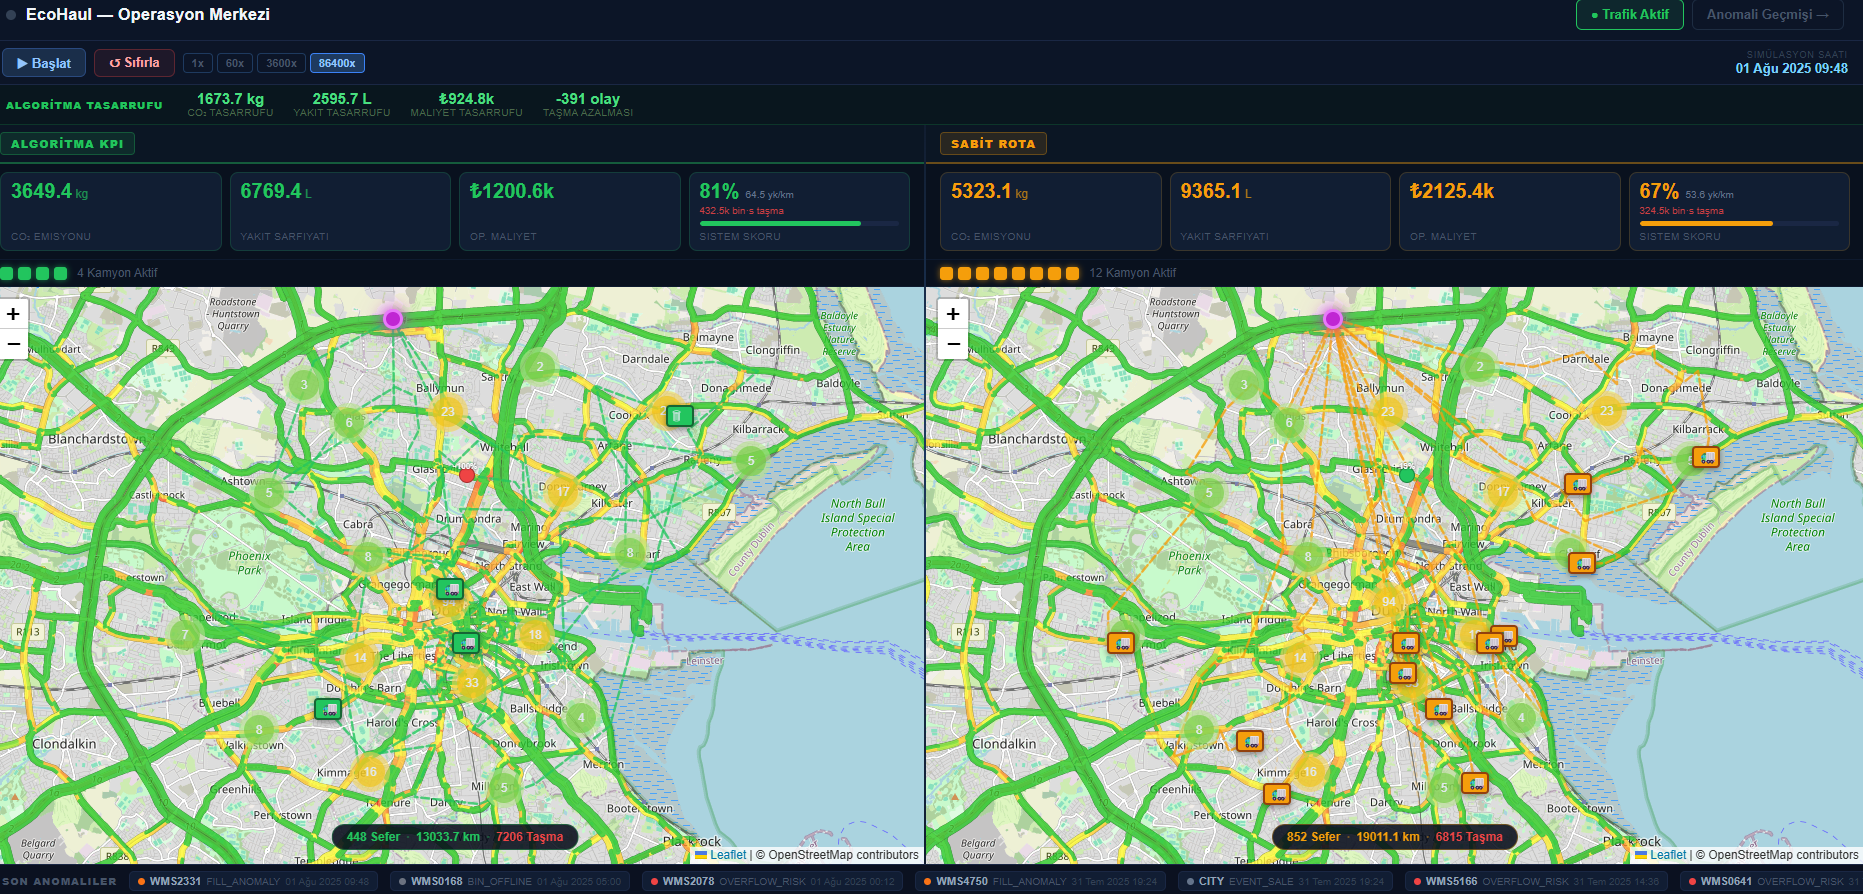
\includegraphics[width=\columnwidth,keepaspectratio]{images/simulation_dashboard.png}
\caption{EcoHaul real-time operations dashboard during a parallel run. Left: the DPET world serves the city at 81\% efficiency with a small active fleet. Right: the fixed-route baseline runs near its fleet ceiling at 67\%. Each side shows colour-coded bin markers, animated trucks, and a live KPI comparison panel.}
\label{fig:dashboard}
\end{figure}

\section{Experimental Evaluation}
\label{sec:eval}
\subsection{Setup}
DPET is compared against two baselines under identical conditions: \textit{Greedy} (purely reactive nearest-neighbor with no ETF, corridor, or efficiency filter) and \textit{2-opt} (fixed daily routes built by sweep + nearest-neighbor + 2-opt, fired at 06:00). All three share the same dataset, fill distribution, environment, and stochastic events. Key parameters are listed in Table~\ref{tab:config}; each algorithm is run $n=4$ times over a full year (01/01/2024--01/01/2025), compressed to $\approx$6 minutes of wall-clock time by an $86{,}400\times$ speed factor, and the runs are averaged.

\begin{table}[t]
\centering
\caption{Simulation configuration.}
\label{tab:config}
\footnotesize
\begin{tabular}{ll}
\toprule
\textbf{Parameter} & \textbf{Value} \\
\midrule
Duration            & 01/01/2024 -- 01/01/2025 \\
Runs per algorithm  & $n=4$ \\
Bins                & 300 active (from 3{,}424 DCC dataset) \\
Label A / B / C     & 20\% / 50\% / 30\% \\
Max fleet size      & 8 / 10 / 12 / 16 trucks \\
Avg.\ truck speed   & 30 km/h \\
Service time        & 5 sim-min per bin \\
Fuel cost           & 45 TL/L \\
Fixed cost per trip & 2{,}000 TL \\
\bottomrule
\end{tabular}
\end{table}

The fleet ceiling of 12 was chosen so that the baselines reach saturation while DPET rarely does: in practice DPET used 6.9 trucks on average versus 11.5 for the baselines. A much lower ceiling would let the baselines hide their inefficiency; a much higher one would let every algorithm serve all bins and erase the gap.

\subsection{KPI Comparison}
Table~\ref{tab:kpi} reports the averaged KPIs; DPET wins on eight of ten metrics, and Fig.~\ref{fig:savings} quantifies its percentage advantage over each baseline. System efficiency reaches 79.0\% versus 59.2\% and 61.8\%---about 20 percentage points---driven mainly by the ETF weight (\texttt{\_W\_ETF}=0.35), which dispatches high-value loads before bins overflow. Load/km, fuel, CO\textsubscript{2}, cost, fleet, trips, and distance all improve substantially. Cost falls more than fuel (39\% vs 30\%) because the 2{,}000\,TL fixed cost per trip is amortised over 42\% fewer trips.

\begin{table}[t]
\centering
\caption{Average KPIs over one-year simulations (best value in bold).}
\label{tab:kpi}
\footnotesize
\setlength{\tabcolsep}{4pt}
\begin{tabular}{lrrr}
\toprule
\textbf{Metric (direction)} & \textbf{DPET} & \textbf{Greedy} & \textbf{2-opt} \\
\midrule
System efficiency (\%) $\uparrow$        & \textbf{79.0}  & 59.2  & 61.8  \\
Load-per-km efficiency $\uparrow$        & \textbf{63.1}  & 47.4  & 49.6  \\
CO\textsubscript{2} (kg) $\downarrow$    & \textbf{2{,}485} & 3{,}586 & 3{,}412 \\
Fuel (L) $\downarrow$                    & \textbf{4{,}601} & 6{,}622 & 6{,}174 \\
Operational cost (k\,TL) $\downarrow$    & \textbf{829}   & 1{,}373 & 1{,}338 \\
Avg.\ fleet size $\downarrow$            & \textbf{6.9}   & 11.5  & 11.5  \\
Number of trips $\downarrow$             & \textbf{311}   & 537   & 530   \\
Total distance (km) $\downarrow$         & \textbf{8{,}877} & 12{,}807 & 12{,}187 \\
Overflow load (k bin$\cdot$s) $\downarrow$ & 283          & \textbf{226} & \textbf{226} \\
Overflow events $\downarrow$             & 4{,}808        & \textbf{3{,}922} & \textbf{3{,}862} \\
\bottomrule
\end{tabular}
\end{table}

The two metrics where DPET is worse---cumulative overflow load and overflow events---are a deliberate trade-off. DPET intentionally holds back slow-filling Label-C bins (which do not individually justify a dispatch under the efficiency and \texttt{MIN\_DISPATCH} rules) until a coverage rotation or corridor opportunity arises, slightly raising overflow time; in exchange it consumes 30--40\% less fuel. A tier-0 aging mechanism bounds this trade-off by forcing extra dispatches for bins that become truly critical. Fig.~\ref{fig:savings} summarises DPET's percentage advantage over both baselines across all KPIs.

\begin{figure}[t]
\centering
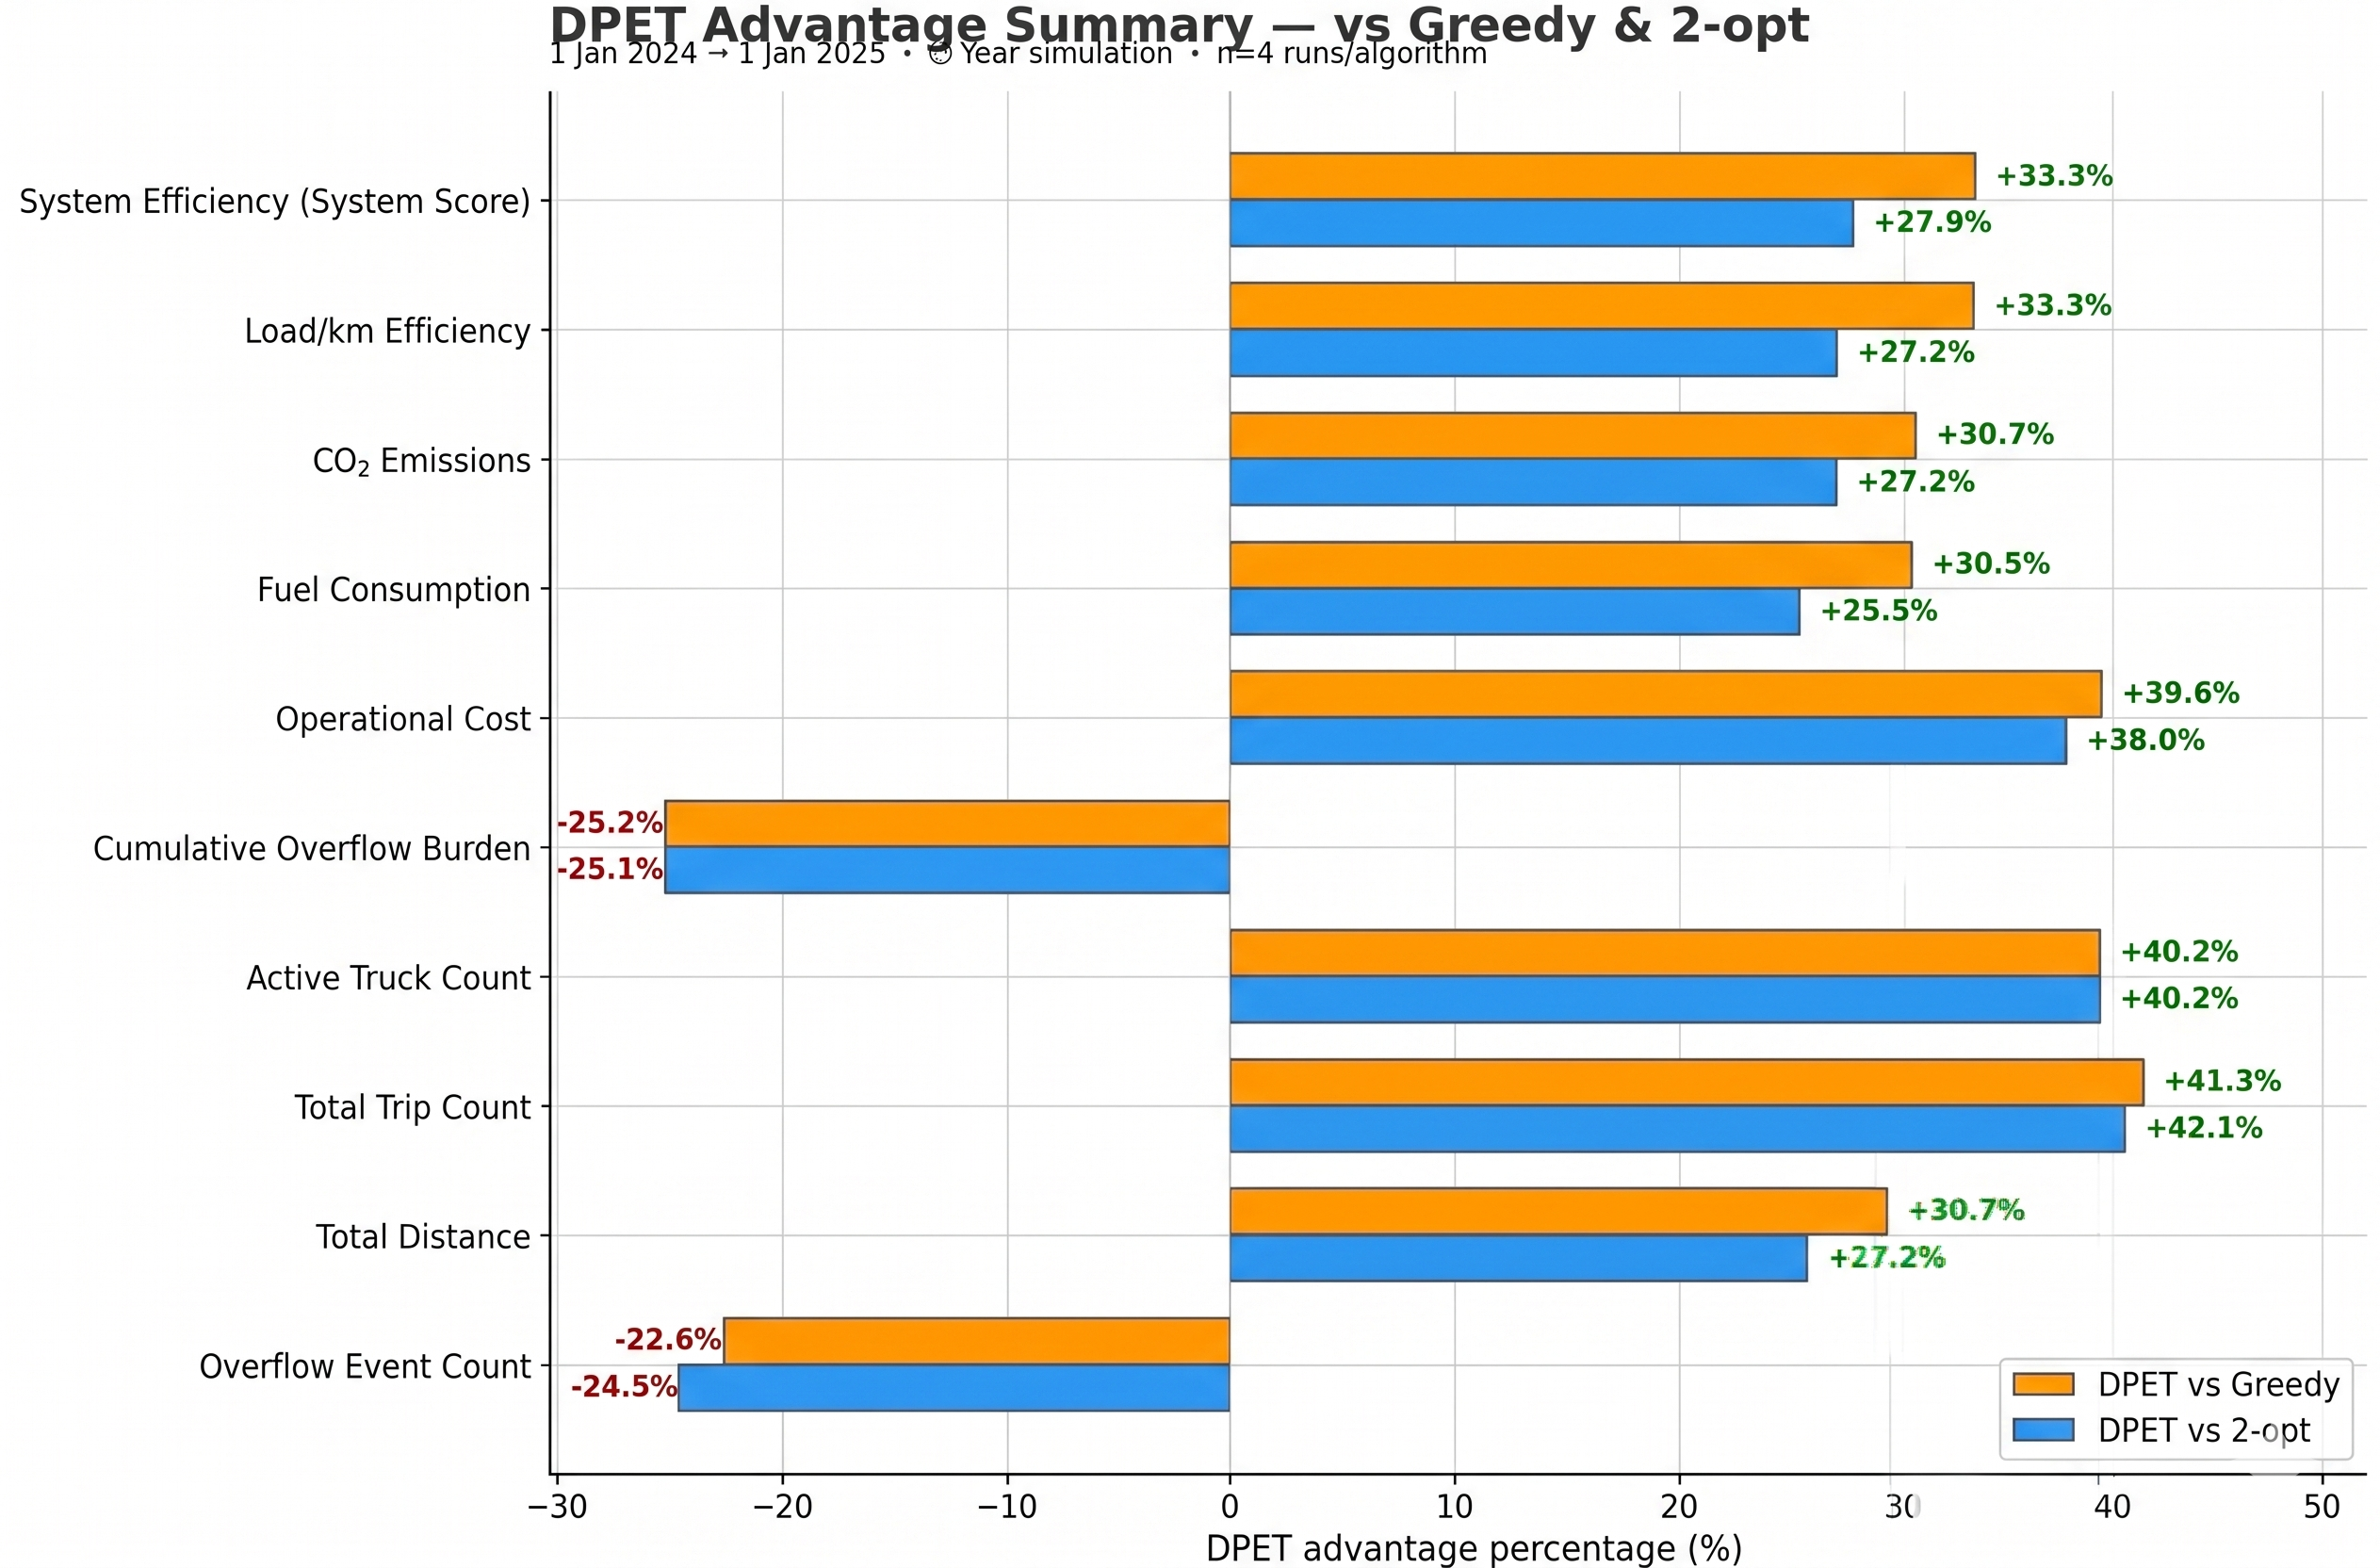
\includegraphics[width=\columnwidth,keepaspectratio]{images/Gemini_Advantage_Summary.png}
\caption{DPET's percentage advantage over the Greedy and 2-opt baselines across all KPIs (positive = DPET better).}
\label{fig:savings}
\end{figure}

\subsection{Efficiency vs.\ Fleet Size}
The clearest behavioural difference appears when efficiency is plotted against the number of trucks (Fig.~\ref{fig:fleet}). DPET operates at 76--87\% efficiency with only 4--7 trucks, and its trend \textit{decreases} as the fleet grows---small fleets already provide full coverage. Greedy rises from 52\% to 66\% only as the fleet grows to 8--16 trucks, and 2-opt spans 57--69\%. In short, a municipality running DPET with 4--7 trucks can beat the best score the baselines reach with 12--16 trucks.

\begin{figure}[t]
\centering
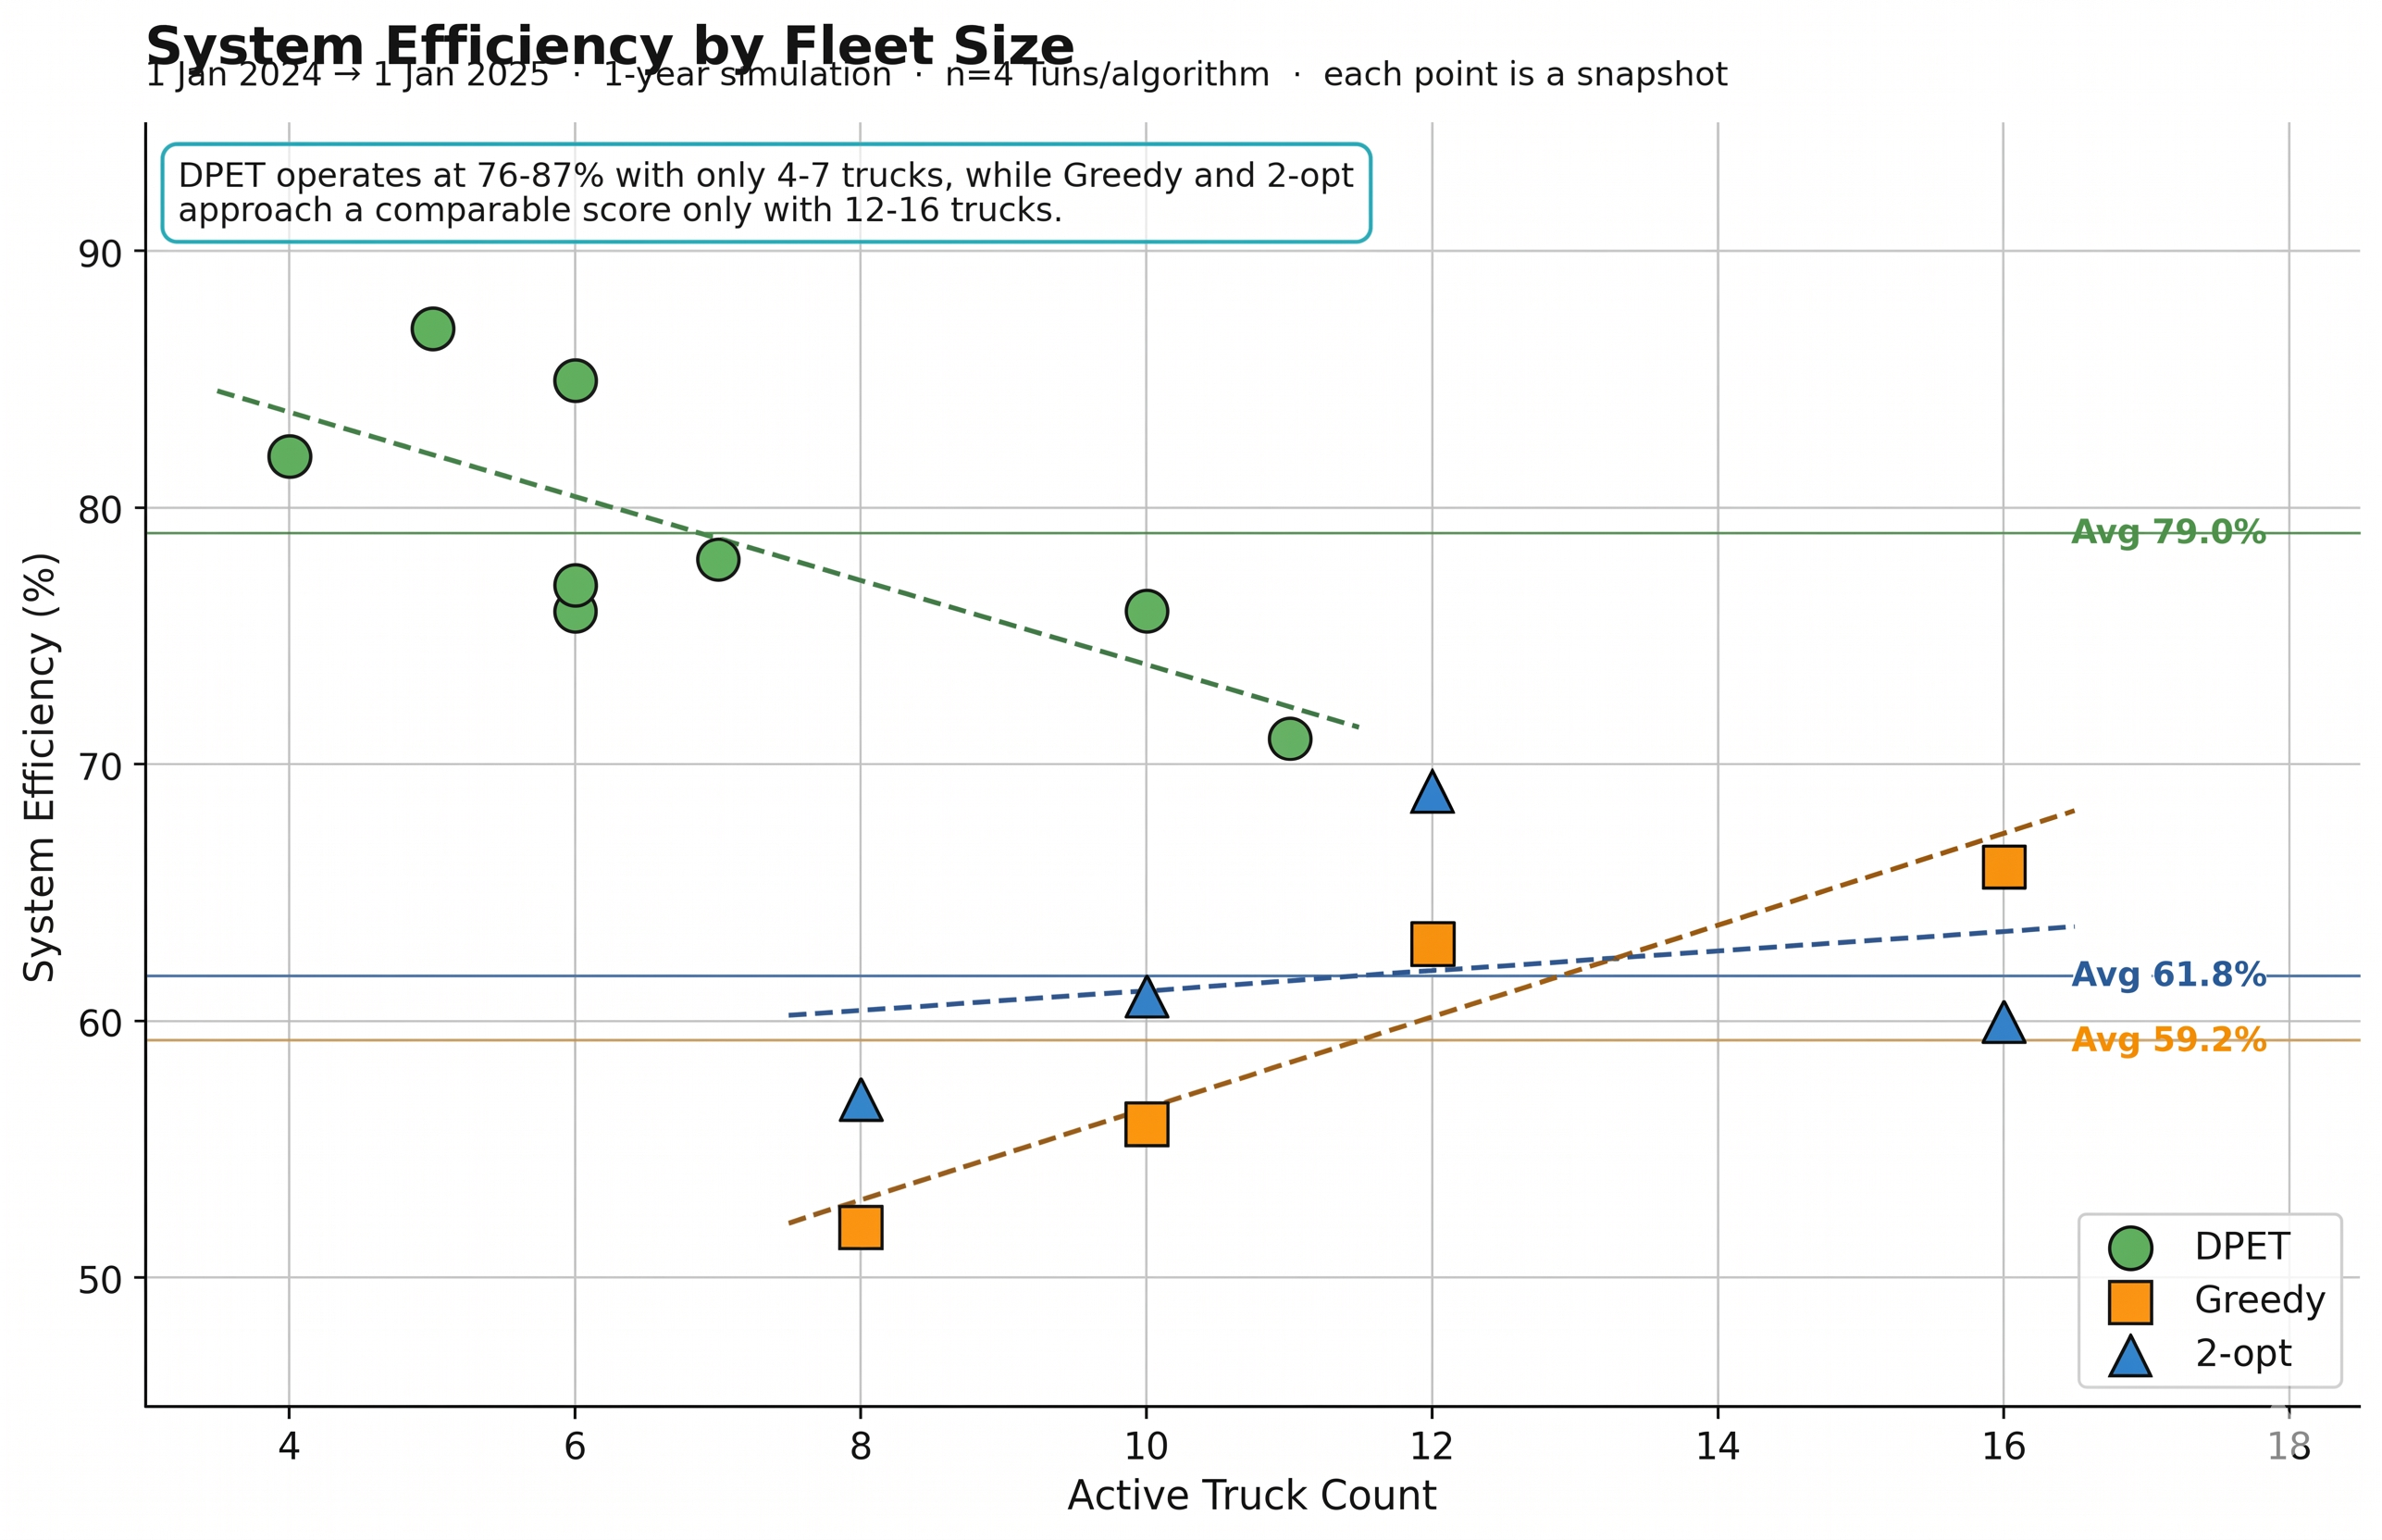
\includegraphics[width=\columnwidth,keepaspectratio]{images/Gemini_Fleet_Size_Average.png}
\caption{System efficiency as a function of the active fleet size. DPET (small fleets) dominates the baselines even at their largest fleets.}
\label{fig:fleet}
\end{figure}

\subsection{Anomaly Detection}
The detector was validated by controlled injection (Table~\ref{tab:anomaly}). Of 125 injected anomalies, 122 were correctly detected (97.6\%). Threshold-clean types (\textsc{overflow\_risk}, \textsc{sensor\_fixed\_value\_error}) reached 100\%. The single missed \textsc{fill\_anomaly} occurred when a bin jumped from empty to full within one tick; the 90\% \textsc{unauthorized\_empty} rate reflects a boundary case at exactly the 100\,m proximity threshold.

\begin{table}[t]
\centering
\caption{Anomaly detection accuracy by category.}
\label{tab:anomaly}
\footnotesize
\begin{tabular}{lrrr}
\toprule
\textbf{Anomaly Type} & \textbf{Injected} & \textbf{Detected} & \textbf{Accuracy} \\
\midrule
OVERFLOW\_RISK             & 50 & 50 & 100.0\% \\
FILL\_ANOMALY              & 20 & 19 & 95.0\% \\
SENSOR\_FIXED\_VALUE\_ERROR & 15 & 15 & 100.0\% \\
BIN\_OFFLINE               & 30 & 29 & 96.7\% \\
UNAUTHORIZED\_EMPTY        & 10 & 9  & 90.0\% \\
\midrule
\textbf{Overall}           & \textbf{125} & \textbf{122} & \textbf{97.6\%} \\
\bottomrule
\end{tabular}
\end{table}

\section{Conclusion and Future Work}
EcoHaul demonstrates the feasibility of an AI-driven smart waste management system grounded in real Dublin bin data. Its contributions are a parallel dual-world simulation enabling rigorous A/B comparison, a six-layer DPET algorithm with mass-aware routing, a proactive ETF/K-means fill predictor, and a unified REST API shared by the simulation and physical IoT sensors. Across one-year simulations, DPET improves system efficiency by $\approx$30\%, cuts fuel and CO\textsubscript{2} by $\approx$28--29\% and operational cost by $\approx$39\%, and serves the same demand with 40\% fewer trucks and 42\% fewer trips than greedy and 2-opt baselines, while the anomaly detector reaches 97.6\% accuracy. Embedding a physics-grounded ($F=m\cdot a$) cost function into the routing optimizer is an original contribution that distinguishes DPET from standard CVRP heuristics.

Several directions can extend EcoHaul from a validated prototype toward a field-deployable smart-city platform.

\textit{Wide-area communication.} The current ESP32 layer uses WiFi, which is adequate for prototyping but impractical at city scale because of its short range ($<$100\,m) and relatively high power draw. Migrating the link to LoRaWAN (868\,MHz ISM band, Class~A) would let a single gateway cover thousands of bins at multi-kilometre range while extending battery life from months to years. Since a fill reading fits in a single byte, LoRaWAN's low bandwidth and duty-cycle limits pose no obstacle, and the migration is architecturally transparent: a network server such as ChirpStack or The Things Network forwards each uplink to the existing \texttt{/api/devices/\{bin\_id\}/state-change} endpoint, so no backend code changes are required.

\textit{Learning-based prediction.} The rolling-average ETF estimator is robust and training-free but statistically naive. As the \texttt{telemetry} and \texttt{event\_log} tables accumulate labelled time series, they become a training set for gradient-boosted trees (LightGBM, XGBoost), seasonal time-series models (SARIMA, Prophet), or deep sequence models (LSTM, Temporal Fusion Transformer) that explicitly capture hour-of-day, day-of-week, weather, and event effects; the current estimator then serves as a baseline. The same data richness would also let the rule-based anomaly detector be upgraded to unsupervised models (Isolation Forest, autoencoder reconstruction error) able to flag previously undefined anomaly types.

\textit{Driver assignment.} EcoHaul currently plans at the level of \textit{routes}; a real operation must also assign each route to a \textit{driver}. A location-aware assignment module could match DPET routes to the nearest available drivers with the Hungarian (Kuhn--Munkres) algorithm, minimising total dead mileage subject to shift constraints, with a reinforcement-learning policy as a longer-term extension that additionally accounts for live traffic, driver fatigue, and predicted route-completion times.

\textit{Automated parameter tuning.} The DPET constants---scoring weights, fill/ETF thresholds, and tier intervals---are presently hand-calibrated. Because they form a rich, mutually interacting parameter space, Bayesian optimization or meta-learning could tune them automatically per city, potentially widening the margin over the baselines without manual effort.

\textit{Real-world deployment.} Finally, a pilot with a small physical bin fleet would validate the simulation's fill and cost assumptions against field measurements and fully close the digital-twin loop, turning EcoHaul from a simulation-validated prototype into an operational municipal system.

\section*{Acknowledgment}
We thank Yeditepe University and the project advisors for their support, and Dublin City Council for the open bin-location dataset.

\balance
\begin{thebibliography}{00}
\bibitem{gutierrez2015} J.\,M.\ Gutierrez, M.\ Jensen, M.\ Henius, and T.\ Riaz, ``Smart waste collection system based on location intelligence,'' \textit{Procedia Computer Science}, vol.~61, pp.~120--127, 2015.
\bibitem{arebey2012} M.\ Arebey, M.\,A.\ Hannan, H.\ Basri, R.\,A.\ Begum, and H.\ Abdullah, ``Solid waste bin level detection using gray level co-occurrence matrix feature extraction approach,'' \textit{Journal of Environmental Management}, vol.~104, pp.~9--18, 2012.
\bibitem{pardini2018} K.\ Pardini, J.\,J.\,P.\,C.\ Rodrigues, S.\,A.\ Kozlov, N.\ Kumar, and V.\ Furtado, ``IoT-based solid waste management solutions: a survey,'' \textit{Journal of Sensor and Actuator Networks}, vol.~8, no.~1, p.~5, 2018.
\bibitem{dantzig1959} G.\,B.\ Dantzig and J.\,H.\ Ramser, ``The truck dispatching problem,'' \textit{Management Science}, vol.~6, no.~1, pp.~80--91, 1959.
\bibitem{christofides1976} N.\ Christofides, ``Worst-case analysis of a new heuristic for the travelling salesman problem,'' Report 388, Graduate School of Industrial Administration, Carnegie Mellon University, 1976.
\bibitem{akhtar2017} M.\ Akhtar, S.\,A.\ Hannan, R.\,A.\ Begum, H.\ Basri, and E.\ Scavino, ``Backtracking search algorithm in CVRP models for efficient solid waste collection and route optimisation,'' \textit{Waste Management}, vol.~61, pp.~117--128, 2017.
\bibitem{anagnostopoulos2015} T.\ Anagnostopoulos, A.\ Zaslavsky, A.\ Kaloxylos, and S.\ Georgakopoulos, ``Robust waste collection exploiting cost efficiency of IoT potentiality in smart cities,'' in \textit{Proc.\ IEEE Int.\ Conf.\ Recent Advances in Internet of Things (RIoT)}, Singapore, 2015, pp.~1--6.
\bibitem{malapur2017} B.\,S.\ Malapur and V.\,R.\ Pattanshetti, ``IoT based waste management: an application to smart city,'' in \textit{Proc.\ IEEE Int.\ Conf.\ Energy, Communication, Data Analytics and Soft Computing (ICECDS)}, 2017, pp.~2476--2479.
\bibitem{grieves2017} M.\ Grieves and J.\ Vickers, ``Digital twin: mitigating unpredictable, undesirable emergent behavior in complex systems,'' in \textit{Transdisciplinary Perspectives on Complex Systems}, F.-J.\ Kahlen et al., Eds.\ Cham: Springer, 2017, pp.~85--113.
\bibitem{zanella2014} A.\ Zanella, N.\ Bui, A.\ Castellani, L.\ Vangelista, and M.\ Zorzi, ``Internet of things for smart cities,'' \textit{IEEE Internet of Things Journal}, vol.~1, no.~1, pp.~22--32, Feb.~2014.
\bibitem{eurostat2022} Eurostat, \textit{Municipal Waste Statistics}, European Commission, Luxembourg, 2022.
\bibitem{dcc2023} Dublin City Council, ``DCC Public Bin Locations Dataset,'' Dublin City Council Open Data Portal, 2023.
\end{thebibliography}

\end{document}
